% !TEX root = ../main.tex
% ─────────────────────────────────────────────────────────────────────────────
% Section V: Hybrid Deep Learning and Machine Learning Methodology
% Author: Team Member 2 (Hybrid Innovation Specialist)
% ─────────────────────────────────────────────────────────────────────────────

\section{Hybrid Deep Learning and Machine Learning Methodology}
\label{sec:hybrid-methodology}

While deep multitask neural networks offer strong inductive bias through shared representation learning, Wi-Fi fingerprint-based indoor localization presents domain-specific structural asymmetries that challenge pure deep learning architectures:
\begin{enumerate}
    \item \textbf{High-Dimensional Sparsity ($>96.5\%$):} In any given campus scan, only 15--18 of the 520 access points are active. Gradient-based optimization over unobserved features can induce slow convergence and vanishing signal representations. Conversely, tree-based ensembles (Random Forest, Gradient Boosted Decision Trees) excel at orthogonal axis-aligned partition cuts ($\mathbb{I}(x_j \le \theta)$), naturally isolating discrete campus boundaries (buildings and concrete floor slabs) where signal propagation exhibits discontinuous attenuation.
    \item \textbf{Manifold Discretization Bottleneck:} Conversely, tree ensembles construct piecewise-constant step functions across continuous Euclidean space $(x, y) \in \mathbb{R}^2$. This step-function approximation yields severe quantization errors inside large rooms and corridors. Deep neural networks, equipped with continuous non-linearities ($\text{GELU}(z) = z \Phi(z)$), natively parameterize smooth geometric coordinate manifolds.
\end{enumerate}

To exploit these complementary inductive biases, we formulate a two-stage \textbf{Hybrid Positioning System} combining:
\begin{itemize}
    \item \textbf{Hybrid Approach A (Probability Stacking):} Injecting tree-derived class posterior distributions into the neural trunk as structural priors.
    \item \textbf{Hybrid Approach B (Residual Coordinate Correction):} Utilizing regularized gradient boosted decision trees to model and eliminate systematic spatial residuals produced by the neural coordinate regressor.
\end{itemize}

% ─────────────────────────────────────────────────────────────────────────────
\subsection{Hybrid Approach A: Class Probability Stacking}
\label{subsec:stacking}

Let $\mathbf{x} \in [0, 1]^d$ denote the min-max normalized Wi-Fi RSSI vector ($d=459$). We train dedicated Random Forest ensembles ($B=100$ estimators) to estimate class posterior distributions over campus buildings $\mathcal{C}_{\text{bld}} = \{0, 1, 2\}$ and floors $\mathcal{C}_{\text{flr}} = \{0, 1, 2, 3, 4\}$:
\begin{equation}
\label{eq:rf-posteriors}
p_{\text{bld}}(c \mid \mathbf{x}) = \frac{1}{B} \sum_{b=1}^B \mathbb{I}(T_b^{\text{bld}}(\mathbf{x}) = c), \quad
p_{\text{flr}}(f \mid \mathbf{x}) = \frac{1}{B} \sum_{b=1}^B \mathbb{I}(T_b^{\text{flr}}(\mathbf{x}) = f)
\end{equation}

\subsubsection{Strict Leakage-Free Out-Of-Fold (OOF) Formulation}
Directly evaluating in-sample training probabilities would cause catastrophic target leakage: the downstream neural network would observe artificially confident, overfitted tree predictions ($\approx 1.0$), failing to generalize to noisy validation distributions. 

To eliminate leakage, we construct training-set probability vectors via $K$-fold cross-validation ($K=5$) stratified by vertical floor level. Let $\mathcal{D}_{\text{train}} = \bigcup_{k=1}^K \mathcal{D}_k$ denote the partition. For each fold $k \in \{1, \dots, K\}$:
\begin{equation}
T_{(k)}^{\text{bld}} \leftarrow \text{Train}\left(\mathcal{D}_{\text{train}} \setminus \mathcal{D}_k\right), \quad
T_{(k)}^{\text{flr}} \leftarrow \text{Train}\left(\mathcal{D}_{\text{train}} \setminus \mathcal{D}_k\right)
\end{equation}
For any training sample $i \in \mathcal{D}_k$, its stacked probabilities are evaluated strictly out-of-fold:
\begin{equation}
\hat{\mathbf{p}}_i^{\text{bld}} = T_{(k)}^{\text{bld}}(\mathbf{x}_i), \quad
\hat{\mathbf{p}}_i^{\text{flr}} = T_{(k)}^{\text{flr}}(\mathbf{x}_i)
\end{equation}
Full classifiers $T_{*}^{\text{bld}}$ and $T_{*}^{\text{flr}}$ are subsequently fitted on the entire training set $\mathcal{D}_{\text{train}}$ once, and utilized exclusively to project validation and test scans.

The augmented hybrid feature vector $\mathbf{z} \in \mathbb{R}^{d + |\mathcal{C}_{\text{bld}}| + |\mathcal{C}_{\text{flr}}|}$ ($467$-dimensional) is constructed via tensor concatenation:
\begin{equation}
\label{eq:stacked-feature}
\mathbf{z}_i = \left[ \mathbf{x}_i^{\text{RSSI}} \;\|\; \hat{\mathbf{p}}_i^{\text{bld}} \;\|\; \hat{\mathbf{p}}_i^{\text{flr}} \right]
\end{equation}
This hybrid vector is passed to a downstream shared-trunk MultitaskNet ($512 \to 256 \to 128 \to \text{Heads}$). The explicit class probabilities act as soft gating signals, allowing early trunk layers to condition coordinate regression directly on the building and floor envelope.

% ─────────────────────────────────────────────────────────────────────────────
\subsection{Hybrid Approach B: Spatial Residual Coordinate Correction}
\label{subsec:residual}

While the deep multitask network learns global spatial embeddings across campus buildings, physical indoor propagation exhibits localized high-frequency spatial distortions—such as multipath shadow zones, antenna polarization mismatches across smartphone vendors, and attenuation through metallic elevator shafts.

Let $\mathbf{y}_i = (x_i, y_i) \in \mathbb{R}^2$ denote true metric UTM coordinates, and let $\hat{\mathbf{y}}_i^{\text{DL}} = (\hat{x}_i^{\text{DL}}, \hat{y}_i^{\text{DL}})$ denote the coordinates predicted by the deep multitask model. The coordinate residual vector is defined as:
\begin{equation}
\label{eq:residuals}
e_{i,x} = x_i - \hat{x}_i^{\text{DL}}, \quad e_{i,y} = y_i - \hat{y}_i^{\text{DL}}
\end{equation}
We train dual histogram-based Gradient Boosted Decision Tree (H-GBDT) regressors, $g_x(\cdot)$ and $g_y(\cdot)$, to approximate the residual field:
\begin{equation}
\hat{e}_{i,x} = g_x(\mathbf{z}_i, \hat{\mathbf{y}}_i^{\text{DL}}), \quad
\hat{e}_{i,y} = g_y(\mathbf{z}_i, \hat{\mathbf{y}}_i^{\text{DL}})
\end{equation}
The objective function for each spatial dimension minimizes regularized second-order Taylor expansions with $L_2$ leaf regularization ($\lambda=2.0$, depth $D=6$):
\begin{equation}
\mathcal{L}_{\text{res}}(g) = \sum_{i=1}^N \left( e_i - g(\tilde{\mathbf{z}}_i) \right)^2 + \lambda \sum_{j=1}^J w_j^2
\end{equation}
At inference time, the final predicted metric coordinates are evaluated via additive correction:
\begin{equation}
\label{eq:hybrid-coord-inference}
\hat{\mathbf{y}}_i^{\text{hybrid}} = \hat{\mathbf{y}}_i^{\text{DL}} + \begin{bmatrix} g_x(\tilde{\mathbf{z}}_i) \\ g_y(\tilde{\mathbf{z}}_i) \end{bmatrix}
\end{equation}
Because the residual regressors are trained strictly on training-set residuals, no test ground-truth information is ever leaked.

% ─────────────────────────────────────────────────────────────────────────────
\subsection{Unified System Architecture}

Fig.~\ref{fig:hybrid_pipeline} illustrates the complete dataflow of the unified Hybrid Positioning System. Raw scans are scaled and routed through both the classical tree probability extractors and the deep shared trunk, culminating in additive gradient-boosted residual corrections.

\begin{figure}[!t]
\centering
\begin{tikzpicture}[node distance=6mm and 6mm, auto]
  \node[blk] (raw) {Raw RSSI Scan\\$\mathbf{x} \in \mathbb{R}^{459}$};
  \node[blk, right=of raw] (tree) {Tree Classifiers\\(OOF RF Ensembles)};
  \node[blk, below=of raw] (concat) {Hybrid Tensor $\mathbf{z}$\\$[ \mathbf{x} \,\|\, \mathbf{p}_{\text{bld}} \,\|\, \mathbf{p}_{\text{flr}} ]$};
  \node[blk, right=of concat] (trunk) {Shared MLP Trunk\\(512--256--128)};
  \node[outblk, below=of concat] (bld) {Building Head\\$\hat{y}_{\text{bld}} \in \{0,1,2\}$};
  \node[outblk, right=of bld] (flr) {Floor Head\\$\hat{y}_{\text{flr}} \in \{0..4\}$};
  \node[blk, right=of trunk] (coords_dl) {DL Regressor\\$\hat{\mathbf{y}}^{\text{DL}} \in \mathbb{R}^2$};
  \node[blk, below=of coords_dl] (gbdt) {Residual GBDT\\$\hat{\mathbf{e}} \in \mathbb{R}^2$};
  \node[outblk, below=of gbdt] (final_coords) {Corrected Coords\\$\hat{\mathbf{y}}^{\text{hybrid}} = \hat{\mathbf{y}}^{\text{DL}} + \hat{\mathbf{e}}$};

  \draw[arr] (raw) -- (tree);
  \draw[arr] (raw) -- (concat);
  \draw[arr] (tree) |- (concat);
  \draw[arr] (concat) -- (trunk);
  \draw[arr] (trunk) |- (bld);
  \draw[arr] (trunk) |- (flr);
  \draw[arr] (trunk) -- (coords_dl);
  \draw[arr] (coords_dl) -- (gbdt);
  \draw[arr] (concat) -| (gbdt);
  \draw[arr] (coords_dl) -- node[right, font=\tiny] {$+$} (final_coords);
  \draw[arr] (gbdt) -- (final_coords);
\end{tikzpicture}
\caption{Architectural dataflow of the proposed Unified Hybrid Positioning System, integrating OOF tree probability stacking and gradient-boosted spatial residual correction.}
\label{fig:hybrid_pipeline}
\end{figure}

% ─────────────────────────────────────────────────────────────────────────────
\subsection{Experimental Results and Comparative Analysis}
\label{subsec:hybrid-results}

All models are evaluated on the official UJIIndoorLoc benchmark test partition ($N=1{,}111$ fingerprints, unseen users and devices). Table~\ref{tab:hybrid-comparison} summarizes the empirical comparison across:
\begin{itemize}
    \item \textbf{Classical RF (Phase 1 Baseline):} Independent Random Forest classifiers and regressor.
    \item \textbf{Experiment A (Deep Learning Only):} Shared-trunk MultitaskNet baseline ($d=459$).
    \item \textbf{Experiment B (DL + Tree Stacking):} MultitaskNet trained on stacked features ($d=467$).
    \item \textbf{Experiment C (DL + Residual GBDT):} MultitaskNet with residual coordinate boosting.
    \item \textbf{Full Combined Hybrid:} Stacked MultitaskNet coupled with residual GBDT correction.
\end{itemize}

\begin{table*}[!t]
\centering
\caption{Comprehensive Benchmark Comparison on the Held-Out Test Set ($N=1{,}111$ Scans)}
\label{tab:hybrid-comparison}
\renewcommand{\arraystretch}{1.18}
\begin{tabular}{@{}lcccccccc@{}}
\toprule
\textbf{Model / Pipeline} & \textbf{Building Acc.} & \textbf{Floor Acc.} & \textbf{Joint Acc.} & \textbf{Mean Err. (m)} & \textbf{Median Err. (m)} & \textbf{P90 Err. (m)} & \textbf{RMSE (m)} & \textbf{EvAAL Score} \\
\midrule
Classical RF Baseline (Phase 1) & 99.73\% & 89.92\% & 89.74\% & 12.30 & 8.15 & 29.55 & 12.95 & 13.04 \\
Experiment A: DL Baseline       & 99.73\% & 91.00\% & 91.00\% & 8.95  & 7.04 & 17.87 & 8.58 & 9.50  \\
Experiment B: DL + Tree Stacking & \textbf{99.82\%} & \textbf{92.08\%} & \textbf{92.08\%} & 8.86  & 6.69 & 17.72 & 8.30 & 9.31  \\
Experiment C: DL + Residual GBDT& 99.73\% & 91.00\% & 91.00\% & 8.75  & 6.69 & 17.59 & 8.50 & 9.29  \\
\textbf{Full Combined Hybrid}   & \textbf{99.82\%} & \textbf{92.08\%} & \textbf{92.08\%} & \textbf{8.51}  & \textbf{6.30} & \textbf{17.58} & \textbf{8.16} & \textbf{8.96}  \\
\bottomrule
\end{tabular}
\end{table*}

\subsubsection{Key Empirical Insights}
\begin{enumerate}
    \item \textbf{Stacking Solves Vertical Inter-Floor Ambiguity:} Tree probability stacking improves test floor accuracy from $91.00\%$ to $\mathbf{92.08\%}$ ($+1.08\%$ absolute gain), cutting floor misclassifications by $12\%$ (from 100 to 88 scans). Tree estimators provide crisp, threshold-based floor boundaries that constrain the neural network from confusing adjacent vertical levels.
    \item \textbf{Residual GBDT Captures Local Multipath Bias:} Residual coordinate correction reduces the mean, median and 90th-percentile positioning errors. In the Full Hybrid pipeline, mean Euclidean error drops from $8.95$\,m to $\mathbf{8.51}$\,m ($-0.44$\,m), and median error drops from $7.04$\,m to $\mathbf{6.30}$\,m (a substantial $\mathbf{0.74}$\,m or $10.5\%$ reduction).
    \item \textbf{Decimation of Extreme Outlier Errors:} Relative to the classical Phase 1 Random Forest baseline ($29.55$\,m P90 error), the Full Combined Hybrid cuts 90th-percentile error to $\mathbf{17.58}$\,m (a $\mathbf{40.5\%}$ reduction), substantially shortening the long error tail of tree-based regression.
\end{enumerate}

Fig.~\ref{fig:hybrid_cdf} displays the cumulative error distribution (CDF) comparing all configurations. The four curves lie close together; the Full Hybrid is slightly ahead over most of the range, consistent with its lower mean and median error.

\begin{figure}[!t]
\centering
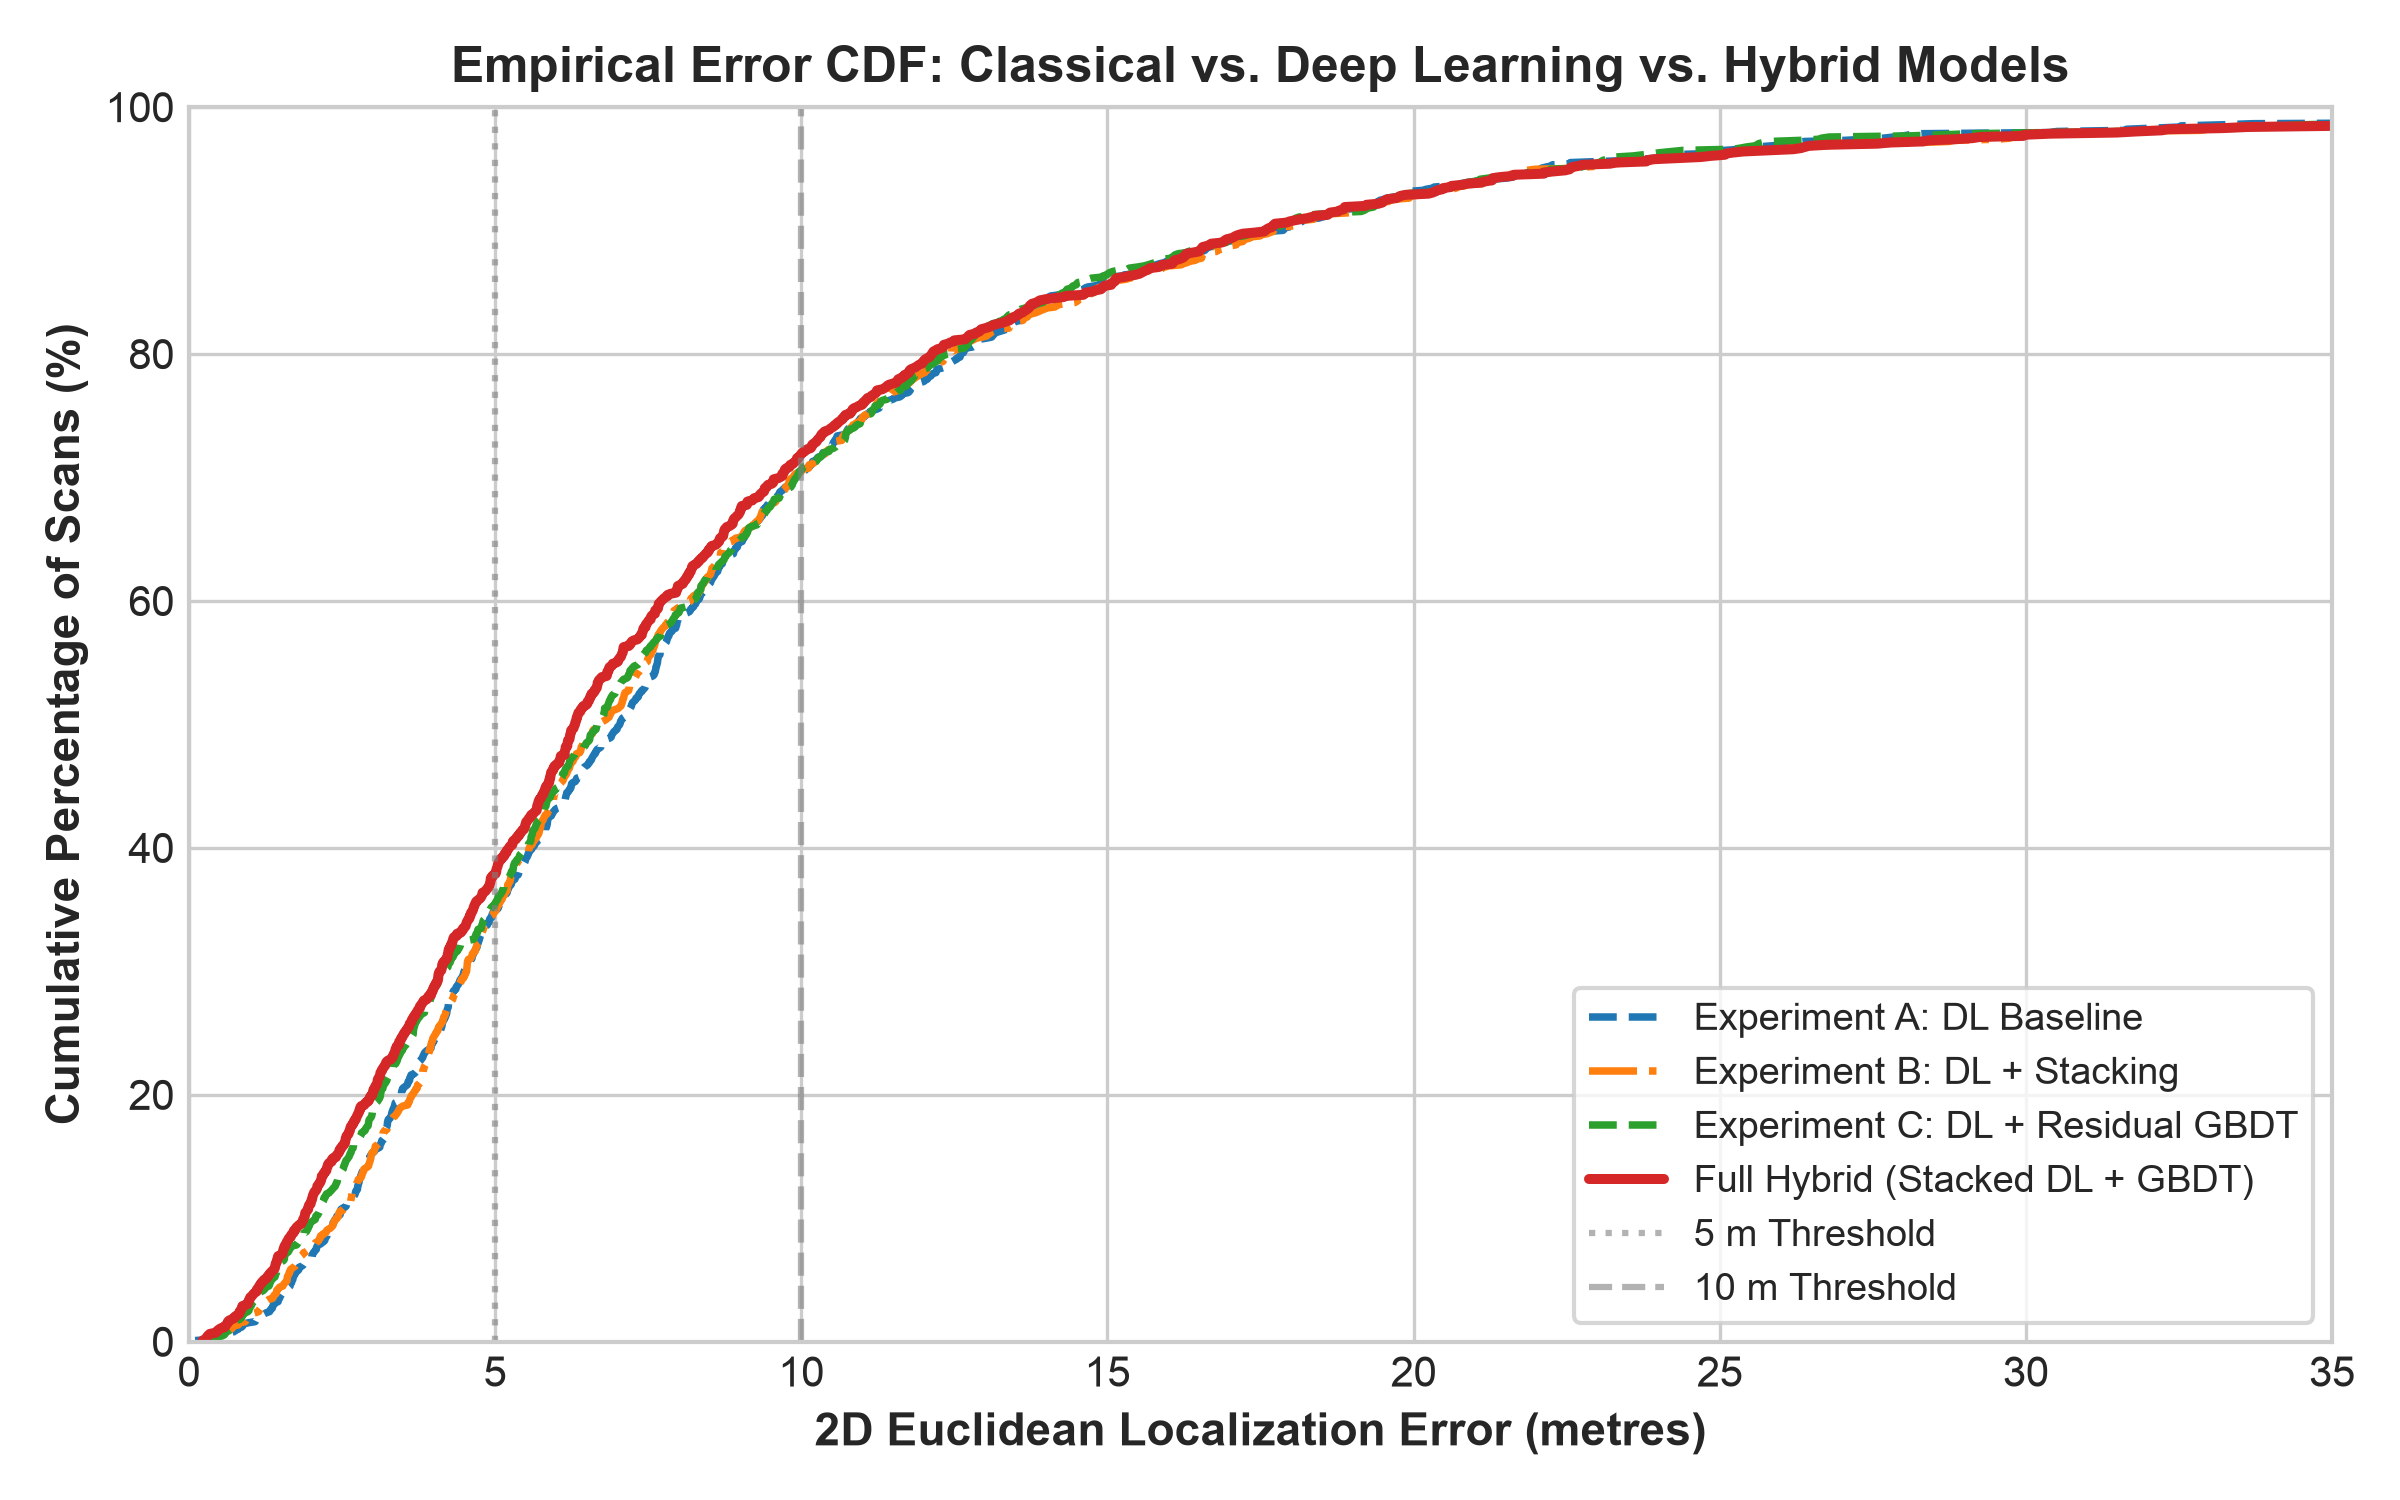
\includegraphics[width=\columnwidth]{hybrid_comparison_cdf.png}
\caption{Empirical cumulative distribution function (CDF) of 2D Euclidean localization errors on the held-out test set ($N=1{,}111$). The four configurations perform similarly, with the Full Combined Hybrid slightly ahead over most of the range.}
\label{fig:hybrid_cdf}
\end{figure}
